\section{Temperature for each month over all the years in Falun}

In these calculations, in figure \ref{fig:measurements}, the temperature average
is measured for all years in Falun (northern Sweden), grouped by the month. The
input to the function that calculates this is the month, and the function
calculates the temperature average and outputs the graph to the screen and to a
file. In order to obtain the graphs for all years the calculation was run for
each month.  Besides the temperature average for each year, the graph also shows
a fitted line over the data.

An interesting observation from the fitted lines on the measurements is that
for the majority of the months the temperature average has been increasing over
the years.


\begin{figure}%
    \centering
    \noindent\makebox[\textwidth]{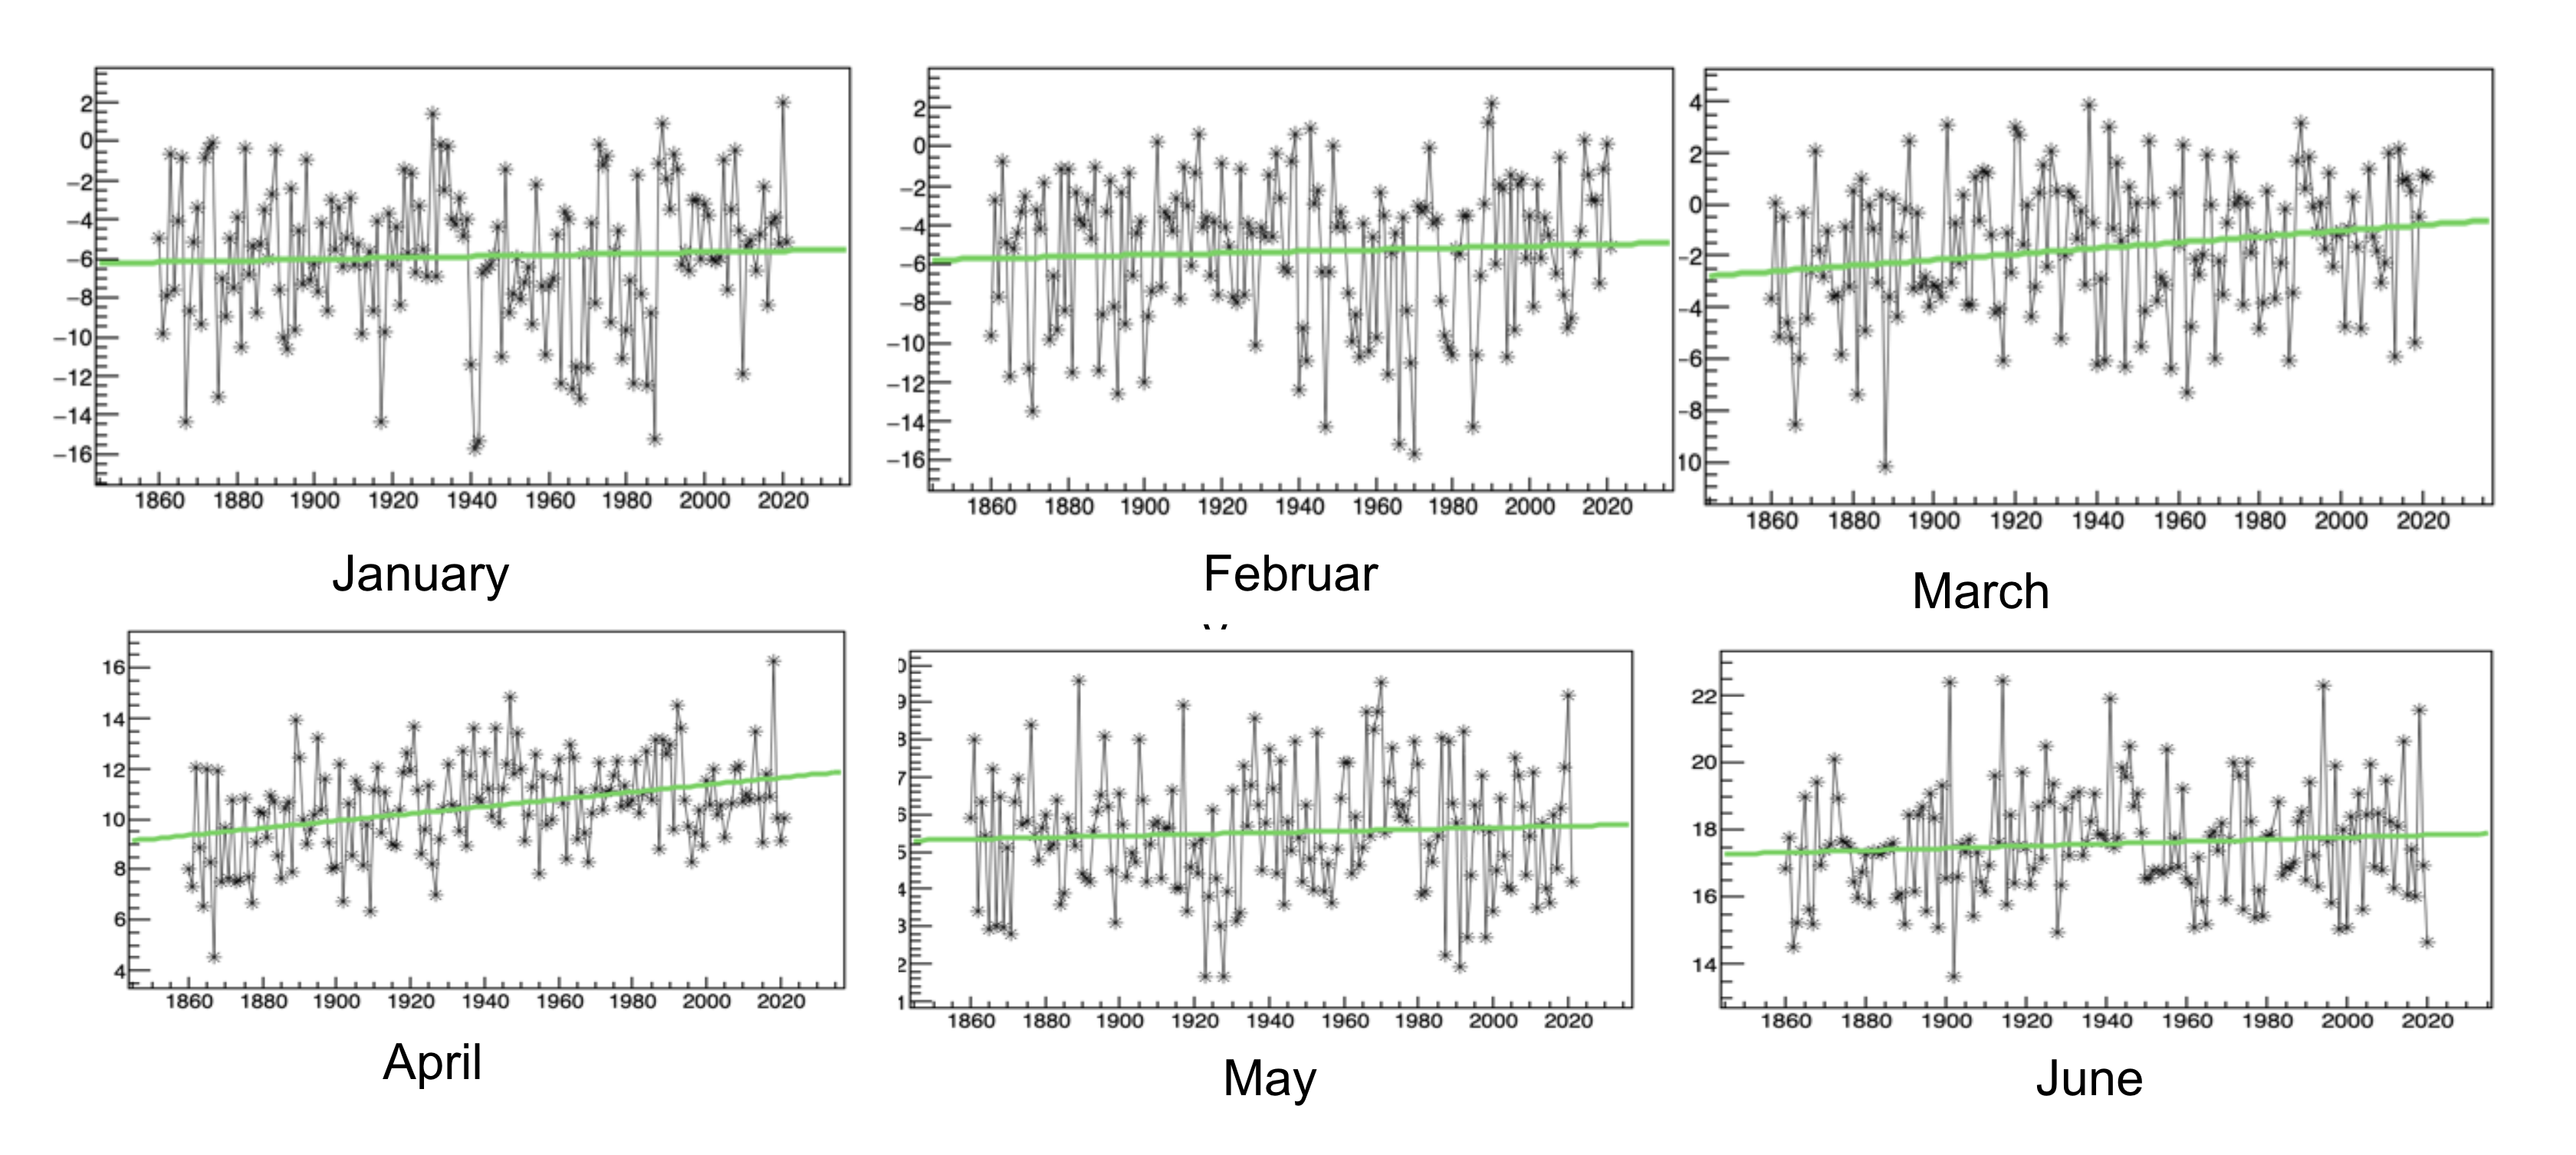
\includegraphics[width=1.6\textwidth]{measurements/images/jan-jun.png}}
    \noindent\makebox[\textwidth]{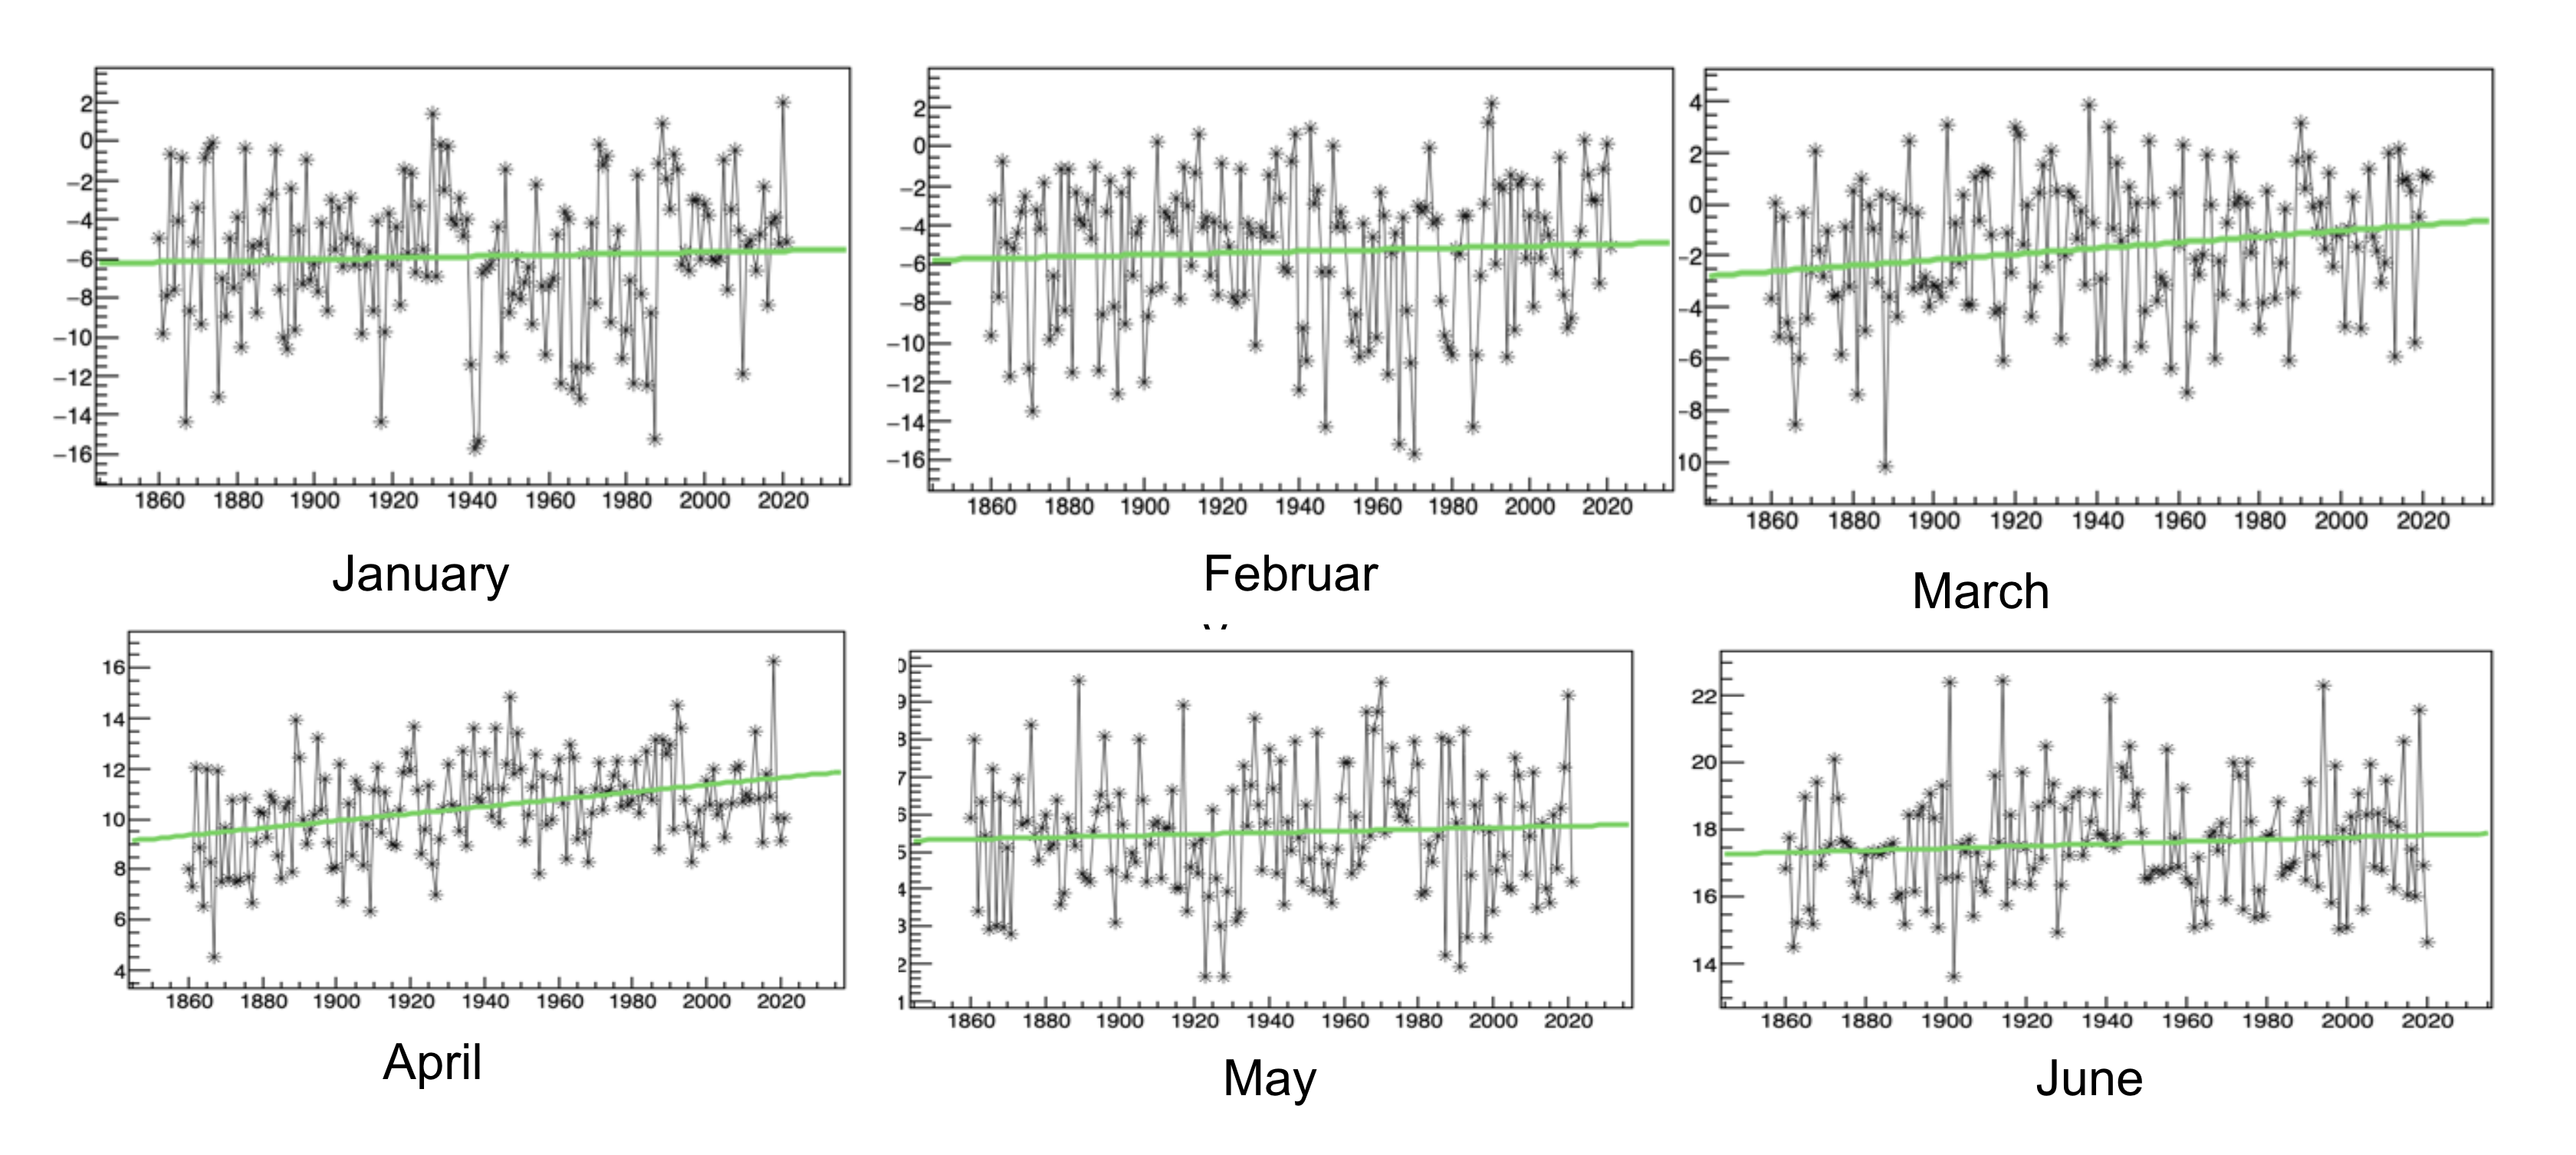
\includegraphics[width=1.6\textwidth]{measurements/images/jan-jun.png}}
    \caption{2 Figures side by side}%
    \label{fig:measurements}%
\end{figure}
